\documentclass[portuguese]{textolivre}
% metadata
\journalname{Texto Livre}
\thevolume{18}
%\thenumber{1} % old template
\theyear{2025}
\receiveddate{\DTMdisplaydate{2025}{1}{16}{-1}}
\accepteddate{\DTMdisplaydate{2025}{3}{18}{-1}}
\publisheddate{\today}
\corrauthor{Laura Rampazzo}
\articledoi{10.1590/1983-3652.2025.57003}
%\articleid{NNNN} % if the article ID is not the last 5 numbers of its DOI, provide it using \articleid{} commmand 
% list of available sesscions in the journal: articles, dossier, reports, essays, reviews, interviews, editorial
\articlesessionname{articles}
\runningauthor{Rampazzo}
%\editorname{Leonardo Araújo} % old template
\sectioneditorname{Daniervelin Pereira}
\layouteditorname{Saula Cecília}

\title{Teletandem no Brasil: uma descrição dos cenários de aprendizagem em instituições brasileiras}
\othertitle{Teletandem in Brazil: a description of learning scenarios at Brazilian institutions}

\author[1]{Laura Rampazzo~\orcid{0000-0002-4736-9900}\thanks{Email: \href{mailto:laura.rampazzo@unesp.br}{laura.rampazzo@unesp.br}}}
\affil[1]{Universidade Estadual Paulista Júlio de Mesquita Filho (UNESP), São Paulo, SP, Brasil.}

\addbibresource{article.bib}

\begin{document}

\maketitle
\begin{polyabstract}
\begin{abstract}
O teletandem caracteriza-se como uma proposta de intercâmbio virtual (IV), uma reconhecida iniciativa pedagógica que conecta estudantes de idiomas que estão distantes geograficamente a fim de que compartilhem suas línguas e culturas. Com trajetória de quase 20 anos de aplicação, o projeto foi pioneiramente proposto na Universidade Estadual Paulista (Unesp) e tornou-se o modelo de IV mais popular no contexto brasileiro, sendo hoje ofertado nas cinco regiões brasileiras. A fim de apresentar uma descrição dos cenários de aprendizagem do teletandem nas instituições do Brasil para que se tenha uma visão abrangente de sua aplicação, foram investigados 45 trabalhos publicados entre 2021 e 2024 e as características que compõem os cenários foram identificadas. Os resultados sugerem que a iniciativa conecta principalmente estudantes universitários em parcerias de português-espanhol e português-inglês, é sustentada pelos princípios delineados por \textcite{vassallo2006} e composta pelas macrotarefas sessão oral de teletandem e sessão de mediação. A aplicação do modelo difere-se, sobretudo, quanto às microtarefas e recursos que são utilizados.

\keywords{Telecolaboração. Aprendizagem de línguas. Contato intercultural. Cenário de aprendizagem. Cenário pedagógico}
\end{abstract}

\begin{english}
\begin{abstract}
Teletandem is a renowned Virtual Exchange (VE) practice that connects geographically distant students of languages so that they exchange their languages and cultures. The project was introduced at São Paulo State University (Unesp), where it has been applied for almost 20 years. It has become the most popular VE model in Brazil, and having spread throughout the country, it is now present in all five Brazilian regions. This paper presents a description of the teletandem learning scenarios in Brazilian institutions to obtain a comprehensive view of its application. The study investigates 45 works published between 2021 and 2024 and identifies the characteristics that compose the scenarios. The results suggest that the initiative mainly connects university students in Portuguese-Spanish and Portuguese-English partnerships, is supported by the principles outlined by \textcite{vassallo2006}, and is composed of the macro-tasks teletandem oral session and mediation session. The application of the model differs, above all, in terms of the micro-tasks and resources used.

\keywords{Telecollaboration. Language learning. Intercultural contact. Learning scenario. Pedagogical scenario}
\end{abstract}
\end{english}
\end{polyabstract}

\section{Introdução}\label{introducao}
Intercâmbio virtual (IV) ou telecolaboração \footnote{Para uma revisão dos termos que foram comumente utilizados para fazer referência a tais práticas, ver \textcite{odowd2018}, entre outras publicações. Atualmente, o termo mais recorrente é intercâmbio virtual \cite{odowd2021}.} pode ser caracterizado como “uma abordagem que promove a interação entre grupos de aprendizes de diferentes países, por meio da integração de uma sequência de tarefas colaborativas e interculturais no currículo de cursos de graduação e pós-graduação” 
\cite[p. v, tradução própria]{ramoscarvalho2023}.\footnote{No original: \begin{english}“an approach that provides interaction between groups of learners from different countries, through the integration of a series of virtual and intercultural collaborative tasks into the curricula of undergraduate and graduate courses”\end{english} \cite[p. v]{ramoscarvalho2023}.} De fato, IVs colocam-se como reconhecidas iniciativas pedagógicas\footnote{Ainda que a pandemia de Covid-19 tenha impulsionado o uso de tecnologias digitais no ensino \cite{athanasiou2024} e de IVs \cite{dooly2022,helm2020,rubin2023,}, os primeiros registros de práticas telecolaborativas são do final do século XX \cite{warschauer1996}.} que, promovidas a partir da aplicação bem-sucedida das tecnologias digitais ao ensino \cite{aranha2023}, conectam estudantes regularmente matriculados em instituições em seus países, os quais colaboram na realização de tarefas com fins de aprendizagem \cite{barbosa2023, cavalari2018, dooly2022, sadler2016}.

IVs são também comumente situados como propostas que objetivam promover a aprendizagem de línguas e a competência intercultural \cite{bozhinova2024, gonzalez-lloret2024, lewis2016, oliveira2024}, frequentemente sendo explorados como estratégias que promovem a internacionalização em casa \cite{calvo2024, koris2023, lee2022, rubinguth2015, salomao2022}.

Conquanto haja algum consenso quanto aos elementos que são essenciais para caracterizar uma iniciativa como IV \cite{rampazzamoore2024b, stevens2021}, seus objetivos de aprendizagem podem ser diversos e as características contextuais têm um impacto no desenho das propostas, as quais podem assumir tipologias e configurações distintas \cite{anikina2015, bozhinova2024, oliveira2024}. IV é, portanto, como pontua \textcite{rubin2023}, um termo mais abrangente para fazer referência a tais iniciativas que, conforme ganham contornos mais particulares, vão sendo reconhecidas por terminologias específicas.

Os programas conforme modelo desenvolvido pela SUNY COIL Center\footnote{\url{https://coil.suny.edu/}. Acesso em 16 dez, 2024.}, por exemplo, são reconhecidos pelo termo COIL, acrônimo para  \textit{Collaborative Online International Learning} \cite{rubinguth2015}, enquanto que a Associação Brasileira de Educação Internacional (FAUBAI) passou a apoiar a implementação do \textit{BRaVE, Brazilian Virtual Exchange}\footnote{\url{https://faubai.org.br/projetos/brave/}. Acesso em 16 dez, 2024.}, nas instituições associadas \cite{salomao2020}. Já os IVs promovidos pela Coordenadoria de Ensino Superior de Graduação (Cesu) do Centro Paula Souza possuem um desenho específico que os caracteriza como Projetos Colaborativos Internacionais (PCIs)\footnote{\url{https://cesu.cps.sp.gov.br/wp-content/uploads/2020/06/VEm-com-PCI-n1-jun-jul-2020.pdf}. Acesso em 16 dez, 2024.}  \cite{succi2020}, ao passo que a aprendizagem telecolaborativa baseada no tandem \cite{brammerts1996}, que foi proposta pioneiramente na Universidade Estadual Paulista (UNESP), é reconhecida como Teletandem\footnote{\url{https://teletandembrasil.org/}. Acesso em 16 dez, 2024.} \cite{telles2006a}.

O teletandem, amplamente divulgado e implementado no Brasil e no exterior, como pontuam \textcite{aranha2021} e \textcite{zakir2022}, é definido como “um modo de telecolaboração -- um contexto virtual, colaborativo e autôno\-mo para a aprendizagem de línguas em que dois estudantes se auxiliam na aprendizagem de suas línguas ou língua de proficiência” \cite[p. 604, tradução própria]{telles2015}.\footnote{No original: \begin{english}“Teletandem is 
a mode of telecollaboration -- a virtual, collaborative and autonomous context for learning foreign 
languages in which two students help each other to learn their own languages 
(or language of proficiency)\end{english}” \cite[p. 604]{telles2015}.} Nesse contexto de promoção do contato intercultural e da aprendizagem de línguas, falantes de diferentes idiomas conectam-se por meio de tecnologias digitais que também permitem a interação síncrona por voz e vídeo, enquanto são acompanhados por seus professores ou mediadores treinados.

A longa trajetória do projeto, que vem sendo implementado há quase 20 anos na UNESP \cite{cavalari2018} e sua expansão para outras instituições no Brasil \cite{aranha2021, lopes2022, munoz2022, rampazzamoore2024, reno2024, souza2020} ressaltam sua relevância no contexto acadêmico brasileiro e o tornam a proposta telecolaborativa mais popular no país \cite{barbosa2023} a julgar pela extensa produção acadêmica de seus pesquisadores, como discutido por \textcite{aranha2021}, \textcite{rampazzacunha2021} e \textcite{aranha2022}.

Como todo IV assume características particulares a depender de seu contexto e dos recursos tecnológicos que estão disponíveis, também as práticas de teletandem se adaptam às necessidades das diferentes turmas e às influências tecnológicas e contextuais \cite{aranha2021, cavalari2022, ferro2024, sartori2021}. \textcite{cavalari2018} já havia demonstrado que a implementação do teletandem tem sido ajustada conforme as especificidades contextuais no âmbito da UNESP e \textcite{aranha2021}, com maestria, traçaram um panorama geral do teletandem em diferentes instituições no Brasil no período de 2010 a 2020. Ainda assim, com o objetivo de situar o projeto como estratégia de promoção do Brasil e de sua(s) cultura(s), o trabalho concentrou-se em identificar as instituições brasileiras e a quantidade de alunos atendidos no período e, até o momento, não parece haver nenhuma investigação que se volte a descrever as características de implementação da proposta de \textcite{telles2006a} nos diferentes contextos institucionais no Brasil. No entanto, compreender como esse modelo de IV é adaptado em diversos contextos importa para que sejam pensadas as estratégias para otimizar seu potencial, inclusive para orientar aplicações em novos contextos, e informar decisões mais eficazes para o ensino de línguas.

Este trabalho visa, pois, apresentar uma descrição dos cenários de aprendizagem do teletandem nas instituições brasileiras, de modo que se tenha uma visão abrangente de sua aplicação a partir do que relatam seus pesquisadores. Para tanto, considerando o intervalo de tempo entre 2021 e 2024, foram compiladas as características de cada contexto conforme apresentadas pelos pesquisadores em publicações sobre o tema, seja em artigos, capítulos, dissertações, teses, relatórios ou trabalhos de conclusão de curso.

As perguntas que orientam esta investigação são: como se organiza a prática de teletandem nas instituições brasileiras?; Em que medida se aproxima e distancia a aplicação do teletandem nas diferentes instituições quanto aos elementos que caracterizam um cenário de aprendizagem?\footnote{O conceito de cenário de aprendizagem será detalhado na próxima seção. Em linhas gerais, corresponde à atualização daquilo que foi planejado para um contexto de aprendizagem. No caso dos IVs, inclui o registro de informações sobre participantes, cumprimento de tarefas e ocorrências.}

Além desta introdução, este artigo divide-se em quatro outras seções. Nas próximas duas, são apresentados o referencial teórico que embasa a proposta do teletandem e sua descrição e os procedimentos metodológicos adotados. Em seguida, discutem-se os resultados e as considerações finais.



\section{Teletandem: princípios, modalidades, tarefas e o conceito de cenário}\label{secao2}
O teletandem \cite{telles2006a}, como mencionado anteriormente, é fruto da adaptação para contextos virtuais do modelo tandem de aprendizagem de línguas e a prática, sobretudo, das habilidades orais \cite{little1996, funk2017}.\footnote{Diversos trabalhos traçam um panorama da evolução do tandem ao teletandem, dentre os quais \textcite{aranha2021}, \textcite{garcia2015}, \textcite{garcia2022}, \textcite{dutra2024} e \textcite{ferro2024}.} Ainda que, em algumas publicações, o teletandem seja equiparado às iniciativas de e-tandem \cite{odowd2018, gonzalez-lloret2024}, enquanto este é comumente utilizado para fazer menção a propostas que promovem o contato assíncrono entre aprendizes, a literatura em teletandem ressalta necessariamente a sincronicidade das trocas (ver, dentre outros, \textcite{aranha2014, messias2020, souza2020}), além do contato assíncrono ocasionalmente para a realização de tarefas específicas \cite{cunha2024, rampazzo2024}.

Marcadamente idealizado para democratizar o acesso ao desenvolvimento de competência comunicativa e cultural àqueles que têm restritas as possibilidades de acesso a cursos e intercâmbios físicos \cite{telles2006a}, a proposição do teletandem no início do século XXI foi bastante inovadora no contexto de um país que apenas uma década antes havia tido o acesso público à internet \cite{paiva2008}, tendo se desenvolvido concomitantemente a outras iniciativas que ganharam projeção internacional, como o COIL. Sua proposta envolve a formação de duplas de falantes de línguas distintas que, por determinado período, encontram-se virtualmente em sessões orais de teletandem\footnote{Também chamado de interação, sessão de interação e sessão de teletandem. Corresponde ao encontro síncrono, de duração determinada, por videoconferência.} por videoconferências para colaborarem no estudo de suas línguas.

Desde seu desenho inicial, o projeto adere aos princípios do tandem de reciprocidade e autonomia. Assim, os participantes não só se alternam nos papéis de aprendizes de uma língua e falantes proficientes de outra, como investem igualmente na aprendizagem do parceiro (reciprocidade) e são responsáveis por tomarem suas decisões quanto ao seus objetivos de aprendizagem e estratégias e por avaliarem a si mesmos e a experiência em um processo negociado com seu par (autonomia) \cite{aranha2014, aranha2021, cappellini2020, garcia2017, moore2023, salomao2009, vassallo2006}.

Além desses, nas publicações de autores brasileiros, a natureza bilíngue das trocas é comumente considerada como um princípio à parte – o princípio de separação de línguas, que, enfatizado por \textcite{vassallo2006}, ressalta a necessidade de que os participantes falem alternadamente os dois idiomas de uma parceria. Os trabalhos subsequentes ao dos autores também tendem a pontuar a necessidade de que os participantes dediquem igualmente o mesmo tempo para a prática de cada um dos idiomas. Recentemente, no entanto, o princípio e, mais especificamente, o termo “separação de línguas” vêm sendo questionados \cite{lima-lopes2023, oliveira2024, picolietal2020, satar2023}.

Ao analisar as sessões orais, \textcite{picolietal2020} identificaram frequentes ocorrências de alternância de códigos (\textit{codeswitching}) e argumentam em favor de uma nova nomenclatura: “princípio da igualdade”. Segundo as autoras, “igualdade” reflete o esforço dos participantes para praticarem a língua alvo ao mesmo tempo em que se afasta de uma concepção monolíngue da comunicação.

Em outra publicação, \textcite{satar2023} sugerem a nomenclatura de “princípio da translinguagem” para que melhor contemple o fato de que os participantes têm à sua disposição -- e fazem uso de -- recursos semióticos para construírem sentido e garantirem a manutenção da conversação em um contexto colaborativo. Os autores enfatizam que esse princípio deve ser interpretado como um guia para a divisão do tempo em que os participantes se alternam em seus papéis, num movimento que se aproxima da compreensão do princípio de reciprocidade de \textcite{brammerts1996}, em que a ação de dedicar a mesma quantidade de tempo a cada idioma aparece incorporada à reciprocidade. Embora não adote um novo termo, \textcite{oliveira2024} também se aproxima do conceito de translinguagem. Ao notar o frequente uso de espanhol em parcerias de português-inglês, a autora enfaticamente defende “o trânsito entre os repertórios linguísticos como um recurso a ser mobilizado e não como uma proibição” (p. 178) e aponta a inadequação do princípio de separação de línguas.

\textcite{lima-lopes2023}, por sua vez, não oferecem nova nomenclatura para o princípio e embora, como \textcite{oliveira2024}, desta\-quem a presença de outros idiomas como estratégia de manutenção da conversação, argumentam que há observação ao princípio de separação de línguas. Segundo os autores, uma vez que os participantes superam as barreiras na comunicação a partir do uso de outros idiomas, voltam a utilizar a língua-alvo. Tal interpretação é igualmente adotada por \textcite{moore2023} na análise de seus resultados, que sugerem que, mesmo quando se apoiam em outros recursos e idiomas, essas estratégias não isentam os participantes de tentarem ser responsáveis à aprendizagem um do outro e equilibrar o uso das duas línguas.

Além dos princípios, como no tandem \cite{brammerts2002}, uma característica que descreve a organização do teletandem segundo sua institucionalização e integração a um curso é a identificação das modalidades. Conquanto possa ser não institucional, isto é, ser desenvolvido fora de uma instituição, desde sua proposição \cite{telles2006a}, o teletandem pode ser reconhecido como institucional, pois, promovido por instituições de ensino, “é viabilizado com o apoio da instituição (que oferece meios para achar um parceiro, espaço físico para interações, recursos técnicos, materiais, apoio de professores-mediadores)” \cite[p. 187]{aranha2014}.

O teletandem institucional, por sua vez, divide-se nas modalidades integrada, semi-integrada e não-integrada \cite{aranha2014, cavalari2018}. O teletandem institucional integrado não só é reconhecido pelas duas instituições às quais os participantes estão vinculados, como ainda é parte integrante dos cursos de línguas em que estão matriculados; assim, os estudantes são avaliados por sua participação e a prática de teletandem é alimentada pelas aulas e vice-versa. Na modalidade semi-integrada, a integração acontece apenas em um dos lados da parceria, assim, enquanto em um contexto institucional os participantes cumprem as atividades como requisito de suas aulas de línguas, do outro, são voluntários que não têm vínculo formal com um curso do qual teletandem faça parte. Por fim, a modalidade não-integrada prevê a realização do teletandem de forma independente de um curso nos dois países.

Independentemente da modalidade, como toda proposta de intercâmbio virtual se organiza em tarefas \cite{rampazzamoore2024b, odowd2009}, também o teletandem o faz. Em uma descrição detalhada das tarefas que ocorrem em um contexto de teletandem institucional integrado, \textcite{aranha2017} ilustram as macro e microtarefas comuns, isto é, as tarefas de maior escopo associadas aos objetivos gerais do projeto, de promover a aprendizagem de línguas e culturas em um processo reflexivo (macro) e aquelas de menor duração que sustentam e apoiam a realização das tarefas em geral (micro).

\begin{figure}[htbp]
  \centering
  \begin{minipage}{.75\textwidth}
    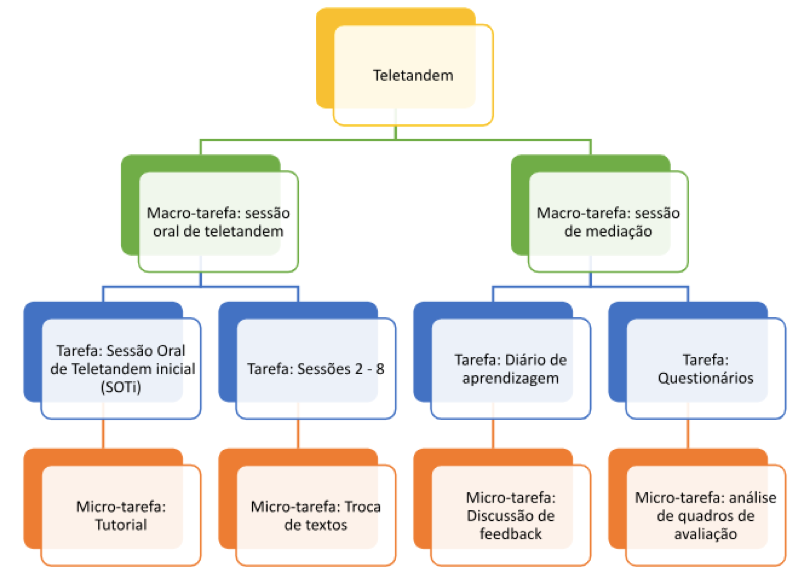
\includegraphics[width=\linewidth]{fig-001.png}
    \caption{Tarefas comuns no teletandem institucional integrado.}
    \label{fig-001}
    \source{\textcite{aranha2017}, tradução de \textcite{rampazzo2021}.}
  \end{minipage}
\end{figure}

Como exemplificado na \autoref{fig-001}, o contexto de teletandem tende a envolver a realização de sessões orais de teletandem (SOTs), que correspondem aos encontros virtuais síncronos possibilitados por ferramentas de videoconferência e duração determinada,\footnote{A duração é variável, mas atualmente costuma durar o período de uma aula de 50 minutos.} e sessões de mediação que, podendo ser conduzidas de maneiras diversas \cite{campos2021}, habitualmente são reuniões realizadas em grupo para promover a reflexão sobre questões do contato intercultural e da aprendizagem de línguas, incluindo 

\begin{quote}
a reflexão de estratégias e táticas de aprendizagem, avaliação sobre o processo de aprendizagem, sobre os princípios do tandem (autonomia, reciprocidade e uso das línguas) e, especialmente, para a troca de ideias, dificuldades, perguntas, e experiências entre os pares \cite[p. 85, tradução própria]{elstermann2022}.\footnote{No original: \begin{english}“reflection on learning strategies and tactics, on evaluation of the learning process, on the principles of tandem learning (autonomy, reciprocity, and language use), and especially on the exchange of ideas, difficulties, questions, and experiences between the participating peers”\end{english} \cite[p. 85]{elstermann2022}.}
%\cite[p. 4]{donaldknuth1984}.
\end{quote}


Assim, a mediação coloca-se como tarefa fundamental para fomentar a aprendizagem reflexiva, assegurando a observação do propósito pedagógico do teletandem. De modo a amparar a reflexão, os participantes ainda escrevem diários de aprendizagem, que favorecem o desenvolvimento da autonomia enquanto os aprendizes refletem sobre suas experiências nas SOTs e questionários, nos quais ponderam seus objetivos e avaliam a experiência. Adicionalmente, associadas às SOTs, também costuma ter a realização de reunião tutorial, na qual a proposta é apresentada aos participantes, bem como suas responsabilidades, e tarefas de troca de textos, escritos na língua-alvo para serem revisados pelos parceiros e reescritos \cite{aranha2014}.

<<<<<<< HEAD
Além dessa descrição das tarefas, \textcite{aranha2017} também usam do conceito de cenário pedagógico descrito por \textcite{chanier2016} para caracterizar aquilo que é planejado para cada novo grupo de participantes no teletandem. Segundo as autoras, em contextos de aprendizagem on-line, o conceito de cenário pedagógico descreve: o ambiente como um todo; os participantes; as atividades e os papéis de cada participante nelas; a ordem das atividades; os recursos que serão utilizados e produzidos; e as instruções que governam as atividades de aprendizagem. No teletandem, adicionalmente inclui o número de macrotarefas e sua tipologia, isto é, se SOTs ou sessões de mediação. Quando se atualiza na prática, o cenário pedagógico passa a ser descrito como cenário de aprendizagem (\textcite{aranha2017}, com base em \textcite{foucher2010}), refletindo o que de fato aconteceu na parceria de teletandem. O cenário de aprendizagem inclui ainda informações sobre os participantes, registro de realização das tarefas e relatos adicionais sobre o que aconteceu.

Com base no entendimento de \textcite{aranha2017}, em alguns contextos, as categorias que caracterizam os cenários pedagógico e de aprendizagem no teletandem passaram a integrar documentos, que funcionam como metadados que descrevem o que foi idealizado para a parceria e o que aconteceu (ver também \textcite{lopes2019}). \textcite{rampazzamoore2024b}, apoiando-se em \textcite{aranha2017} e nos descritores de IVs da \textcite{stevens2021}, sustentam que essas categorias servem para o planejamento e avaliação de IVs e, aqui, argumento que também podem contribuir para que tenhamos uma visão geral do teletandem nos diversos contextos institucionais brasileiros.
=======
Além dessa descrição das tarefas, \cite{aranha2017} também usam do conceito de cenário pedagógico descrito por \textcite{chanier2016} para caracterizar aquilo que é planejado para cada novo grupo de participantes no teletandem. Segundo as autoras, em contextos de aprendizagem on-line, o conceito de cenário pedagógico descreve: o ambiente como um todo; os participantes; as atividades e os papéis de cada participante nelas; a ordem das atividades; os recursos que serão utilizados e produzidos; e as instruções que governam as atividades de aprendizagem. No teletandem, adicionalmente inclui o número de macrotarefas e sua tipologia, isto é, se SOTs ou sessões de mediação. Quando se atualiza na prática, o cenário pedagógico passa a ser descrito como cenário de aprendizagem (\textcite{aranha2017}, com base em \textcite{foucher2010}), refletindo o que de fato aconteceu na parceria de teletandem. O cenário de aprendizagem inclui ainda informações sobre os participantes, registro de realização das tarefas e relatos adicionais sobre o que aconteceu.

Com base no entendimento de \textcite{aranha2017}, em alguns contextos, as categorias que caracterizam os cenários pedagógico e de aprendizagem no teletandem passaram a integrar documentos, que funcionam como metadados que descrevem o que foi idealizado para a parceria e o que aconteceu (ver também \textcite{lopes2019}). \textcite{rampazzamoore2024b}, apoiando-se em \textcite{aranha2017} e nos descritores de IVs da \textcite{stevens2021}, sustenta que essas categorias servem para o planejamento e avaliação de IVs e, aqui, argumento que também podem contribuir para que tenhamos uma visão geral do teletandem nos diversos contextos institucionais brasileiros.
>>>>>>> 9e461e9c156cb04fc53be9851c7ea40967ed5e98


\section{Metodologia}\label{metodologia}

O presente trabalho, de abordagem qualitativa, caracteriza-se como uma pesquisa secundária e descritiva \cite{paiva2019}, uma vez que se vale de dados de pesquisas já divulgadas para caracterizar o atual cenário da prática de teletandem em instituições de ensino formal no Brasil. Para tanto, como complemento ao estudo de \textcite{aranha2021} que se concentrou na quantidade de alunos atendidos e no alcance da oferta de teletandem no Brasil entre 2010 e 2020, este trabalho faz um levantamento das pesquisas que descrevem o contexto de teletandem publicadas no Brasil ou internacionalmente entre 2021 e 2024. Essa escolha é justificada pela necessidade de atualizar o conhecimento sobre a prática, trazendo um panorama dos últimos anos e considerando as transformações tecnológicas, sociais e pedagógicas.

As pesquisas que informam esta investigação foram selecionadas a partir da busca em duas plataformas de bases de dados: Web of Science (WoS) e Google Scholar (GS). Por um lado, a primeira plataforma retorna resultados confiáveis, no sentido de que são estudos publicados em periódicos revisados por pares; no entanto, uma vez que muitas publicações sobre o tema não estão em periódicos indexados à WoS, os resultados não incluem diversos estudos. Por isso, a opção pela busca também no GS que, embora possa trazer resultados duplicados ou não relacionados ao tema, também encontra publicações de outra natureza, como trabalhos de conclusão de curso, dissertações, teses, livros e capítulos, além de artigos publicados em periódicos indexados em outras bases de dados.

A partir da busca pelas palavras-chave “teletandem” e “Brasil” ou “Brazil”, as plataformas retornaram nove resultados no WoS, dos quais um foi excluído por não fazer referência ao teletandem, e 606 no GS, dentre os quais estavam os nove identificados na primeira base de dados. A fim de definir quais trabalhos seriam incluídos para análise, foi adotado como critério o texto apresentar um estudo empírico que se concentra no contexto de teletandem no Brasil e cujos dados foram coletados em período de, no máximo, 10 anos. Foram também eventualmente incluídos trabalhos que descrevem o contexto, mas nomeiam o projeto de outra forma, desde que fossem embasados no referencial teórico do teletandem. Foram excluídos resultados duplicados, isto é, diferentes itens que faziam menção ao mesmo texto, além de trabalhos que: não descrevem o contexto no Brasil; voltam-se à formação de mediadores ou à mediação sem des\-crever a prática de teletandem como um todo ou as outras tarefas envolvidas; não identificam nominalmente as instituições no Brasil; não trazem resultados de pesquisa empírica; são resumos (não expandidos) de comunicações em eventos; ou que não descrevem suficientemente o contexto de teletandem em suas instituições e, logo, não permitem a reconstituição do cenário de aprendizagem. Assim, 45 trabalhos integram o corpus desta investigação, dos quais 22 artigos, quatro capítulos de livros, nove dissertações de mestrado, oito teses de doutorado, um trabalho de conclusão de curso e um resumo expandido de apresentação em evento.

Quanto aos procedimentos de análise, primeiramente foi feito um mapeamento das instituições que promovem o teletandem, tendo sido identificadas 14 instituições, ao menos 17 unidades de ensino: UNESP -- nos campi de Araraquara, Assis e São José do Rio Preto; ETEC; FATEC; IFF; IFSP; IFSULDEMINAS; UEPB; UFAC; UFCG; UFG; UFPB; UNEB; URCA; USP. Em seguida, a partir da leitura dos trabalhos, foram identificados os elementos que compõem o cenário de aprendizagem da oferta de teletandem descrita em cada estudo, sendo consideradas a definição de teletandem pelos autores dos textos e sua descrição do contexto em que o estudo foi realizado. Concomitantemente à leitura das publicações, foram elaborados quadros de cada texto para descrever os cenários de aprendizagem.

Tais quadros (ver \hyperref[apendice]{Apêndice}) foram elaborados com base nos conceitos de cenário pedagógico e de aprendizagem do teletandem de \textcite{aranha2017} e na discussão desses conceitos para o planejamento e avaliação de IVs por \textcite{rampazzamoore2024b}. Por isso, incluem, além da referência bibliográfica do texto consultado, (i) a instituição de ensino que promoveu o teletandem; (ii) o objetivo da oferta; (iii) os princípios que nortearam a prática; (iv) os estudantes participantes envolvidos; (v) a modalidade institucional; (vi) a tipologia da interação entre participantes, se síncrona, assíncrona, ou ambas; (vii) as ferramentas utilizadas; (viii) os idiomas envolvidos na oferta; (ix) a estrutura da proposta e tarefas sugeridas ou recomendadas; (x) a duração do cenário descrito; (xi) o suporte oferecido aos participantes em seu processo de aprendizagem. Tais critérios correspondem aos elementos que compõem, segundo a teoria, a caracterização de um cenário de aprendizagem.

Uma vez reconstituídos os cenários de aprendizagem, foi possível identificar o que possivelmente se caracteriza como o cenário pedagógico prototípico do teletandem em cada uma das instituições e as aproximações e distanciamentos da prática de teletandem entre os contextos, os quais estão descritos na próxima seção.


\section{Resultados e discussão}\label{resultados}

A reconstituição dos cenários de aprendizagem das 14 instituições (17 campi) envolvidas com a oferta de teletandem no Brasil sugere que, como esperado, apesar das especificidades de cada parceria, há diversos pontos de convergência entre eles, uma vez que estão alinhados aos princípios teórico-metodológicos do tandem e teletandem. Nesta seção, primeiramente, apresento e discuto aquilo que poderíamos considerar o cenário pedagógico prototípico do teletandem no Brasil, isto é, as características que normalmente integram o planejamento da proposta e de como ela está prevista para ser executada. Então, discorro sobre as especificidades que se destacam no contexto brasileiro nos últimos anos.

\begin{figure}[htbp]
  \centering
  \begin{minipage}{.75\textwidth}
    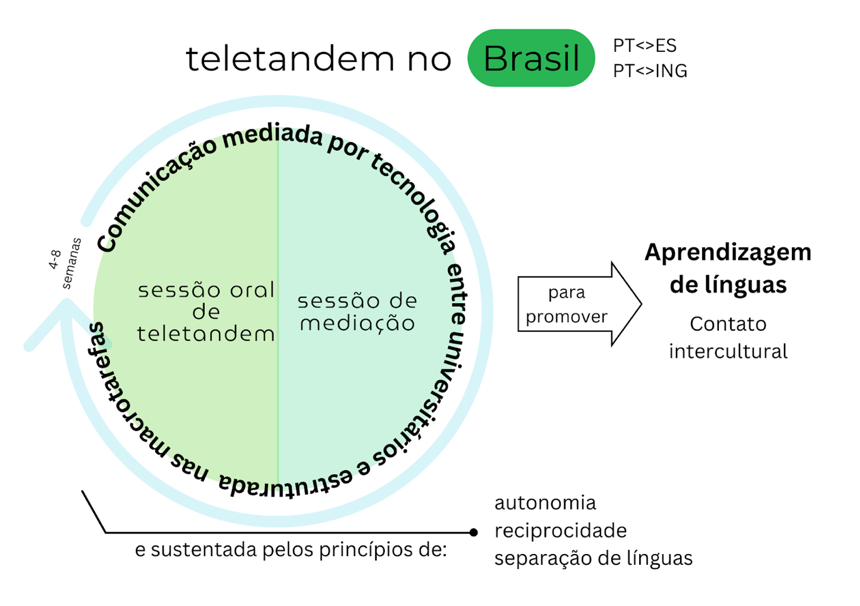
\includegraphics[width=\linewidth]{fig-002.png}
    \caption{O cenário pedagógico prototípico do teletandem no Brasil.}
    \label{fig-002}
    \source{Elaborado pela autora.}
  \end{minipage}
\end{figure}

Ao ilustrar a aplicação do teletandem no país (\autoref{fig-002}), notamos que, nos últimos anos, nas diferentes instituições que o promovem, a proposta se caracteriza por fomentar a comunicação mediada por tecnologias digitais entre estudantes universitários, em sua maioria de graduação, por um período curto -- tipicamente entre 4 e 8 semanas. As parcerias tendem a ser de português-espanhol ou português-inglês e são estruturadas pelas macrotarefas sessão oral de teletandem e sessão de mediação, a fim de possibilitar a aprendizagem de línguas e o contato intercultural, sendo sustentadas pelos princípios de autonomia, reciprocidade e separação de línguas.

Oportunizar a aprendizagem de línguas é o objetivo primário que leva os professores a estabelecerem parcerias com colegas no exterior. A aprendizagem cultural ou o contato intercultural também é um dos propósitos do teletandem, ressaltado em diversas publicações, o que está de acordo com a literatura sobre intercâmbios virtuais, posto que o contato entre pessoas de diferentes culturas tende a ser pressuposto. Adicionalmente, um trabalho, que descreve o contexto da Unesp-Assis, faz menção ao propósito de contribuir para o processo de formação docente, considerando que os participantes faziam licenciatura em Letras \cite{cruz2024}.

Quanto aos idiomas, destacam-se as parcerias de português-espanhol, relatadas em um número maior de contextos (9), seguidas das parcerias de portu\-guês-inglês, em sete instituições.\footnote{As parcerias de português-espanhol são retratadas em 13 publicações, enquanto que as de inglês, em 31. No entanto, há diferentes artigos que investigam o mesmo cenário na mesma instituição.} A esse respeito, ressalto que, a partir dos dados que informam esta investigação, não é possível saber se há mais alunos atendidos em um idioma ou outro, mas o maior número de contextos que promovem a aprendizagem do espanhol sugere que o idioma ganhou proeminência no teletandem. Esse fato pontua a relevância do conhecimento desta língua, sobretudo se considerarmos a localização do nosso país na América Latina e a necessidade de nos prepararmos para a comunicação multilíngue no atual contexto globalizado. Além disso, pode evidenciar os esforços da comunidade acadêmica para a divulgação do idioma, apesar das novas diretrizes para a educação básica terem retirado a obrigatoriedade de seu estudo, por exemplo.\footnote{A Lei nº 14.945/2024, que define as diretrizes para o Novo Ensino Médio, prevê o ensino obrigatório apenas da língua inglesa, ainda que outros idiomas possam ser ofertados, preferencialmente o espanhol \cite{brasil2024}.} Além do espanhol e do inglês, apenas uma outra língua é mencionada: as parcerias de português-alemão na USP \cite{aquino2022}.

Em relação aos princípios, à exceção dos trabalhos resenhados na Seção \ref{secao2} que discutem especificamente o princípio de separação de línguas, majoritariamente, a proposta do teletandem faz referência aos três princípios delineados e nomeados por \textcite{vassallo2006}. Alguns autores, no entanto, optam por bilinguismo ou igualdade, como os que descrevem o teletandem na UEPB (\textcite{maciel2024}\footnote{Conquanto nomeie de “igualdade”, a autora enfatiza que as línguas não devem ser misturadas, o que remete à primeira apresentação dos princípios do teletandem por \textcite{vassallo2006}.}; \textcite{silva2022, silva2022b}) e \textcite{figueiredo2024}, que discute a proposta na UFG, enquanto outros destacam apenas a autonomia e a reciprocidade, como \textcite{pereira2023} da UNEB e \textcite{aquino2022} da USP, o que se aproxima da discussão de \textcite{brammerts1996} e se alinha aos autores no exterior que também não fazem a distinção entre separação de línguas e reciprocidade.

A respeito dessa discussão, há de se apontar que o debate em torno da separação de línguas está ainda primariamente associado a uma questão teórica que, de um lado, enfatiza a necessidade de se considerar o cenário multilíngue e multimodal atual e nega que os participantes sejam proibidos de usar outros recursos e línguas \cite{oliveira2024, satar2023}, mas, de outro, ainda não têm dados que ponderam o que passa a ser efetivamente instruído aos participantes. Assim, considerando o escopo deste trabalho, que pretende ilustrar a prática do teletandem no país, entendo que há a demanda para que, enquanto comunidade, pensemos em como os participantes devem ser orientados. Para além da nomenclatura que iremos utilizar, temos de considerar como prepará-los para o teletandem para que compreendam a natureza bilíngue das trocas, enquanto continuam a fazer uso dos recursos que têm à sua disposição, incluindo outras línguas, para se comunicarem e aprenderem.

Sobre o perfil dos participantes e o contexto da oferta, uma vez que o teletandem é promovido sobretudo em instituições de ensino superior, o público atendido pela proposta também tende a ser de estudantes universitários, de graduação e/ou pós-graduação. Estudantes de ensino médio, porém, também participaram de iniciativas promovidas em instituições de ensino médio e técnico, como a Etec \cite{fernandes2023} e o IFSULDEMINAS \cite{reno2024}. Há a menção ainda a participantes idosos, que participaram desse intercâmbio virtual na Unesp-Assis como parte de um projeto voltado ao público da terceira idade \cite{oliveira2022}.

Nos contextos de ensino superior, o teletandem tem se organizado nas três modalidades institucionais descritas na Seção \ref{secao2}: integrada, semi-integrada e não-integrada. Quando integrado, o projeto faz parte das disciplinas de línguas regulares que compõem a grade curricular obrigatória do curso, enquanto que o semi-integrado e não-integrado costuma envolver participantes voluntários no Brasil de cursos de graduação diversos. Na UEPB e UFG, especificamente, a oferta é integrada a disciplinas eletivas semestrais voltadas para a aprendizagem de línguas e contato intercultural em teletandem.

Já na oferta de teletandem institucional integrado nos Institutos Federais Fluminense (IFF) \cite{willima2021} e Sul de Minas (IFSULDEMINAS) \cite{reno2024}, os participantes não estão matriculados em cursos regulares de graduação ou nível médio, mas, antes, participam da proposta como parte de cursos de idiomas de formação inicial e continuada promovidos pelas instituições. Assim, inscrevem-se voluntariamente no curso de idiomas, mas participam do teletandem de forma mandatória, como requisito do curso.

Quanto à estruturação da proposta, independentemente da modalidade, o projeto tende a envolver as macrotarefas sessão oral de teletandem e sessão de mediação, como na descrição do cenário da Unesp de São José do Rio Preto de \textcite{aranha2017}, ainda que a nomenclatura possa ser diversa. De fato, como aqui, algumas publicações usam o termo sessão oral de teletandem, mas também aparecem os termos sessão de teletandem, sessão de interação, sessão de conversação bilíngue, reunião semanal entre aprendizes, encontro de teletandem, encontro virtual, encontro entre os pares. Igualmente, a sessão de mediação nem sempre é reconhecida assim, mas os estudos referem-se a reuniões que são realizadas por professores que acompanham os participantes.

Aqui, a fim de melhor ilustrar a presença das tarefas nas instituições brasileiras, àquelas com nomes diversos que correspondiam a uma mesma tarefa, adotei a nomenclatura disposta na \autoref{fig-003} e apresentada na seção de revisão da literatura. Como essa figura ilustra, a sessão oral de teletandem, viabilizada por ferramentas de videoconferência (\autoref{fig-004}), necessariamente é prevista e acontece no modelo de intercâmbio virtual do teletandem, já que está descrita nos 45 trabalhos analisados. Esse dado sustenta o que já foi argumentado anteriormente que, embora algumas publicações equiparem parcerias de e-tandem ao teletandem, enquanto o primeiro termo também remete a parcerias que envolvem contatos assíncronos apenas, no teletandem, obrigatoriamente há sessões síncronas por áudio e vídeo.

\begin{figure}[htbp]
  \centering
  \begin{minipage}{.75\textwidth}
    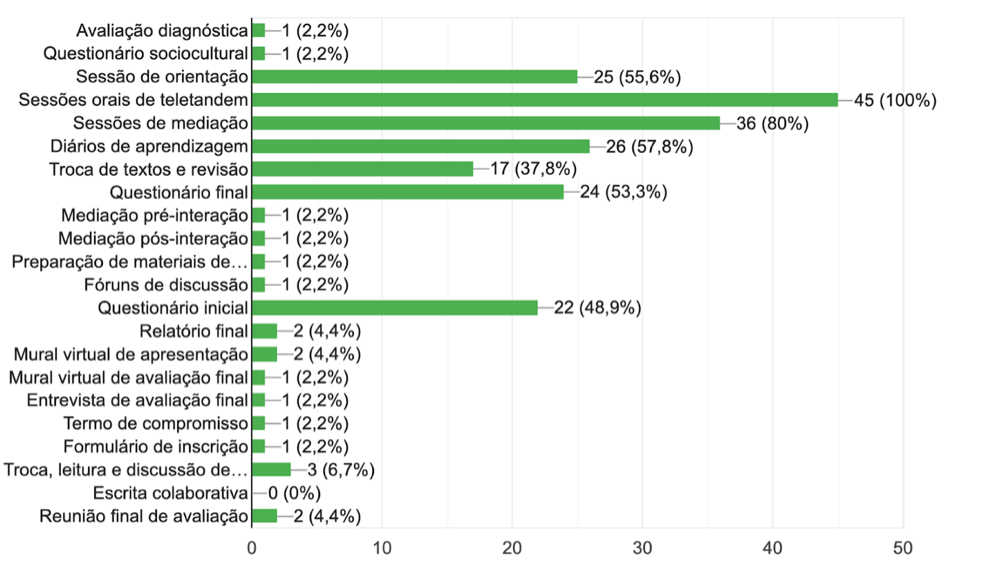
\includegraphics[width=\linewidth]{fig-003.png}
    \caption{Tarefas que ocorrem no contexto de teletandem.}
    \label{fig-003}
    \source{Elaborado pela autora.}
  \end{minipage}
\end{figure}

A sessão de mediação, por sua vez, embora não apareça descrita em todos os trabalhos, é tarefa relevante, estando descrita em 80\% dos trabalhos investigados e em 11 das 14 instituições sob análise. A presença da mediação também sustenta o propósito pedagógico do projeto e o fato de que, como todo intercâmbio virtual, a prática de teletandem é orientada por educadores.

Também comuns são as tarefas que estimulam a reflexão, como diários de aprendizagem e questionários inicial e final, e a reunião de orientação. A menção a outras tarefas como troca de textos escritos na língua-alvo e sua revisão, relativamente frequente nos diferentes contextos, além de tarefas menos frequentes como murais virtuais de apresentação pessoal, fóruns de discussão e preparação de materiais de apoio sobre produções cinematográficas latino-americanas, por exemplo, demonstra que a tipologia das interações que acontecem no teletandem é também assíncrona.

\begin{figure}[htbp]
  \centering
  \begin{minipage}{.75\textwidth}
    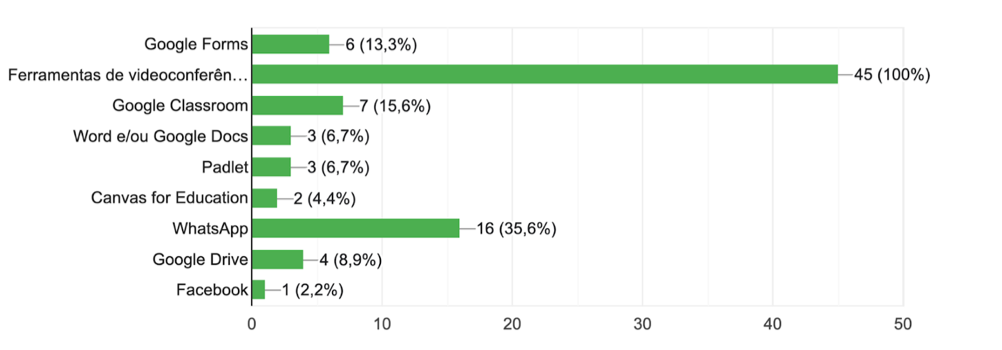
\includegraphics[width=\linewidth]{fig-004.png}
    \caption{Ferramentas de tecnologia digital utilizadas no teletandem.}
    \label{fig-004}
    \source{Elaborado pela autora.}
  \end{minipage}
\end{figure}

Por fim, quanto às ferramentas de tecnologia digital utilizadas (\autoref{fig-004}), nem todas as publicações descrevem os recursos e aplicativos que são utilizados, mas, necessariamente apontam o uso de softwares que possibilitam a conexão síncrona por imagem e voz, sendo mencionados recursos como Google Meet, Zoom e Skype, este último remetendo a dados mais antigos, o que sugere que, atualmente, os dois primeiros são mais comuns. Outra plataforma usual é o WhatsApp, associado principalmente à comunicação entre participantes e mediadores.

Outros recursos como Google Docs, Google Drive, Padlet, Google Forms e Facebook sugerem, como argumentado acima, que algumas tarefas são realizadas de forma assíncrona e a presença de plataformas de gerenciamento da aprendizagem, como Google Classroom e Canvas for Education, indica novamente a orientação que os participantes recebem dos mediadores em seu processo de aprendizagem.

A Tabela \ref{quadro1} a seguir apresenta uma síntese dos principais resultados, com ênfase nos pontos de convergência:

\begin{table}[htpb]
  \centering
  \begin{threeparttable}
    \caption{Síntese dos pontos de convergência entre os cenários de aprendizagem do teletandem no Brasil.}\label{quadro1}
    \begin{tabular}{l l}
      \toprule 
      Categoria do cenário de aprendizagem & Descrição  \\ 
      \midrule
      Objetivos & Aprendizagem de línguas e contato intercultural\\ 
      Princípios & Autonomia, reciprocidade e separação de línguas \\  
      Participantes & Estudantes universitários \\
      Modalidades & Institucional, integrada ou semi-integrada\\
      Tipologia das interações & Necessariamente síncrona\\
      Estrutura das macrotarefas & Sessão oral de teletandem e sessão de mediação\\
      Duração & Curta, tipicamente entre 4 e 8 semanas \\
      Suporte aos participantes & Acompanhados por mediadores \\
      \bottomrule
      \end{tabular}
      \source{Elaborado pela autora.}
  \end{threeparttable}
\end{table}

Em resumo, nos diversos contextos de teletandem no Brasil, há convergência quanto à caracterização geral da proposta, como descrito na Tabela \ref{quadro1}. A aplicação do teletandem distancia-se entre um contexto e outro, sobretudo, quanto aos recursos que são utilizados para prover suporte aos participantes, que são variados, e microtarefas.

\section{Conclusão}\label{conclusao}

A partir do entendimento de que o teletandem é o modelo de intercâmbio virtual mais popular no contexto brasileiro, situando-se como proposta relevante e respeitada por sua longa trajetória no país, este artigo apresentou uma descrição dos cenários de aprendizagem em 14 instituições de ensino brasileiras a fim de identificar (i) como a prática se organiza no Brasil e (ii) em que medida se aproximam e distanciam as práticas nas diferentes instituições.

A identificação dos elementos que compõem os cenários de aprendizagem nas diferentes instituições aponta que, no Brasil, o teletandem tem o objetivo de facilitar a aprendizagem de línguas e o contato intercultural, é apoiado pelos princípios de autonomia, reciprocidade e separação de línguas e, tipicamente, envolve a formação de parcerias entre estudantes universitários, as quais duram algumas semanas. Os idiomas mais comuns são português-espanhol e português-inglês e a prática tende a ser estruturada pelas macrotarefas sessão oral de teletandem e sessão de mediação, o que sustenta a obrigatoriedade da sincronicidade nas interações e a orientação por educadores.

A aplicação do modelo teletandem nas diferentes instituições brasileiras difere-se, sobretudo, quanto às microtarefas que são planejadas e realizadas, além da preferência por uma ou outra ferramenta de tecnologia digital para viabilizar o cumprimento das tarefas e oferecer suporte. Há ainda alguma divergência na nomenclatura das tarefas e no entendimento do princípio de separação de línguas, embora, majoritariamente, os diferentes contextos o reconheçam como um terceiro princípio.

Quanto às limitações deste trabalho, considerando que os dados que informaram a investigação foram obtidos a partir da descrição dos contextos de teletandem em estudos empíricos publicados em diversos formatos, a reconstituição dos cenários de aprendizagem não pôde ser muito detalhada nem incluir dados específicos sobre a quantidade e demografia dos participantes. Adicionalmente, certamente há contextos em que o teletandem tem sido implementado e que, no entanto, não foram ainda divulgados em artigos científicos ou relatórios de prática e, por isso, não estão descritos aqui. Assim, embora as publicações selecionadas permitiram determinar os elementos essenciais que constituem os cenários de aprendizagem e caracterizar o cenário pedagógico prototípico do teletandem no Brasil em uma visão geral, é importante que a comunidade envolvida com a promoção do teletandem no país continue a trabalhar ativamente na divulgação de suas práticas a fim de fortalecer sua oferta e orientar aplicações desse modelo de IV.

\section*{Agradecimento}

Agradeço Viviane Klen-Alves Moore, pela leitura atenta da primeira versão deste trabalho. Suas valiosas sugestões, bem como as dos pareceristas, foram fundamentais para aprimorar a apresentação do texto.

\printbibliography\label{sec-bib}
%conceptualization,datacuration,formalanalysis,funding,investigation,methodology,projadm,resources,software,supervision,validation,visualization,writing,review

\subsection*{Apêndice}\label{apendice}
Este documento apresenta, a partir da adaptação dos conceitos de cenário pedagógico e de aprendizagem do teletandem de \textcite{aranha2017} e na discussão do planejamento de IVs por \textcite{rampazzamoore2024b}, descrições de como essa proposta telecolaborativa vem sendo implementada em instituições brasileiras de ensino. A íntegra do apêndice pode ser consultada neste \href{https://docs.google.com/document/d/1cVHzOuu7kBQe5CfekfkArf91Pd_Lgr8mlCRVzJWYmio/edit?usp=sharing}{\textit{link}}.


\end{document}
